% !TEX encoding = UTF-8
% !TEX TS-program = pdflatex
% !TEX root = ../Lahmer_Abdelilah_tesi.tex
% !TEX spellcheck = it-IT

%**************************************************************

\chapter{La scelta del progetto}

\section{Interesse aziendale negli stage}
%In questa sezione parlerò del tipo di relazione che lega l'azienda al mondo degli stage e il loro interesse per questi. Parlerò inoltre della presenza di altri ex-stagisti che hanno fatto un mio percorso simile e sono stati assunti.

Viste le dimensioni e l'attuale espansione dell'azienda, dovuta anche al momento di buona ripresa economica che sta vivendo l'Italia, Sopra Steria Group S.p.A. è sempre più alla ricerca di nuove figure da inserire nelle proprie divisioni che operano in diversi ambiti e settori.\\

%Le modalità con cui la società attua alla ricerca di risorse sono molteplici, queste infatti possono andare dal reclutamento attraverso agenzie per il lavoro al reclutamento tramite \textit{social network} orientati al lavoro (come ad esempio LinkedIn\footnote{LinkedIn. URL: \url{https://goo.gl/nc4mVh}}), passando per il reclutamento per mezzo di eventi organizzati dalle università o dagli enti pubblici per agevolare l'incontro tra le aziende e gli studenti.\\
%
%Quest'ultimo tipo di evento rappresenta la modalità con cui sono entrato in contatto con Sopra Steria, ovvero grazie al progetto Stage-IT\footnote{Stage-IT. URL: \url{https://goo.gl/UvdwLK}}, nella sua \ang{14} edizione che si è tenuta in data 5 Aprile 2017, dove le aziende hanno avuto modo di esporre i propri progetti e gli studenti le proprie ambizioni a far parte di essi. STAGE–IT infatti è un'occasione di conoscenza reciproca per permettere agli studenti di avvicinarsi al mondo del lavoro e alle imprese di presentare la realtà in cui operano, illustrando le tematiche proposte per stage, con specifico riferimento al settore “\textit{Information and Communication Technology}" (ICT\glossario).\\
%
%	\begin{figure}[H]
%		\centering
%	   	
\includegraphics[width=0.5\textwidth]{immagini/StageIT}
%	   	\caption{StageIT 2017 - Fonte: \url{https://goo.gl/TqV3A6}}
%	\end{figure}


La politica aziendale prevede una durata di sei mesi per completare il ciclo di stage, due di questi considerati curricolari in accordo con l'Università degli Studi di Padova e quattro extracurricolari. Successivamente, nella maggior parte dei casi, vi è la propensione all'assunzione.\\%, in quanto la nuova risorsa si considera pronta per essere effettivamente inserita nei team di sviluppo o di analisi.\\

Il tirocinio è quindi visto dall'azienda come uno strumento utile a contribuire alla selezione di nuovi talenti e verificare che da entrambe le parti vi sia un interesse a proseguire il rapporto lavorativo.\\

L'interesse dell'azienda per gli stagisti e per l'incanalamento di questi nel mondo del lavoro mi è stato confermato una volta approdato nella sede per i colloqui conoscitivi, qui infatti ho avuto modo di rincontrare un collega dell'università che anch'esso aveva seguito lo stesso percorso prima di me. Questo collega infatti dopo aver concluso lo stage curricolare, conseguito la laurea ed aver concluso anche il periodo di stage extracurricolare è stato assunto a tempo indeterminato; l'unica differenza dal percorso che stavo per intraprendere io però è stato soltanto il fatto che questo collega dopo la fine dello stage bimestrale ha chiesto il cambio di \textit{Business Unit} passando alla "792 - Industria e Servizi" dove ha trovato un inquadramento come sviluppatore di applicazioni \textit{web} e \textit{mobile}. Vista questa esperienza l'impressione che l'azienda aveva trasmesso inizialmente si è sempre più confermata e personalmente guardavo con fiducia l'avvenire all'interno di Sopra Steria.

\section{Il progetto all'interno dell'azienda}
%In questa sezione parlerò del progetto che mi è stato proposto dell'azienda.

Gli stage che le aziende proponevano durante l'evento Stage-IT erano prevalentemente orientati a progetti contenuti che secondo le aziende erano fattibili nel \textit{range} di tempo che il corso di studi ci impone, ovvero un minimo di 300 ed un massimo di 320 ore. Dopo aver dato una buona impressione all'evento sono rimasto in contatto con l'amministrazione delle risorse umane di Sopra Steria Group S.p.A, che alla fine del mese di Aprile mi ha convocato per un colloquio collettivo assieme ad altri otto candidati. Anche in questa sede l'impressione che sono riuscito a dare e quella che sono riuscito a percepire da parte dell'azienda è stata più che positiva. Il 17 Maggio infatti iniziavo il mio percorso presso Sopra Steria.\\

Durante il colloquio conoscitivo collettivo le domande sono state varie, in particolare una domanda ha fatto la differenza, ovvero: "Quali sono le vostre ambizioni per il futuro?". Inizialmente lo stage ideale che vedevo in azienda consisteva in un progetto nel ramo della programmazione \textit{mobile}, proiettandomi già in un ottica di stesura di una relazione di fine stage in cui sono portato a presentare un vero e proprio progetto possibilmente, che sarebbe stato sicuramente fattibile in quel ramo. La mia risposta però ha fatto sì che tutto questo venisse sconvolto. La mia replica infatti è stata grossomodo: "La mia ambizione per il futuro è quella di diventare un \textit{Project Manager} oppure un Analista Funzionale, certamente dopo aver fatto un po' di anni di gavetta per acquisire esperienza". Il colloquio collettivo infine si è concluso con la mia convocazione ad un incontro assieme al \textit{Project Manager} di prossimità della sede che mi ha illustrato in maniera generica il progetto su cui lavora il team, ovvero ELISE\glossario, e in cosa consisteva la figura di \textit{Project Manager} e Analista Funzionale in quell'ambito lavorativo. A primo impatto il ramo del \textit{banking} sembrava interessante ma rimanevo comunque aggrappato al mio stage ideale su quello del \textit{mobile}; cosa che però non ha considerato l'amministrazione delle risorse umane, che mi ha indirizzato alla \textit{Business Unit} "793 - Servizi Finanziari e Assicurazioni" con il fine di formare una figura di Analista Funzionale.\\

Lo stage, quindi, così come stava per essere intrapreso, consisteva nella formazione per una mansione più che consistere in un progetto.\\

Assieme al tutor che mi era stato assegnato si sono poi decisi gli obiettivi e a grandi linee il percorso che dovevo seguire. Quest'ultimo prevedeva la mia formazione anche sulle tecnologie e modalità di sviluppo utilizzate lato \textit{back-end}\glossario\ al fine di avere un'ottica più ad ampio raggio sull'intero funzionamento del sistema, sia lato teorico che tecnico.
%Dopo una prima fase di formazione sulle tecnologie ed una di esercitazione secondo i metodi aziendali di sviluppo, quindi, il lavoro di stage si è concentrato su questo software, chiamato ELISE. Ho portato avanti il suo ampliamento aggiungendo le nuove funzionalità il cui sviluppo mi è stato assegnato.
	
%	\begin{figure}[H]
%		\centering
%	   	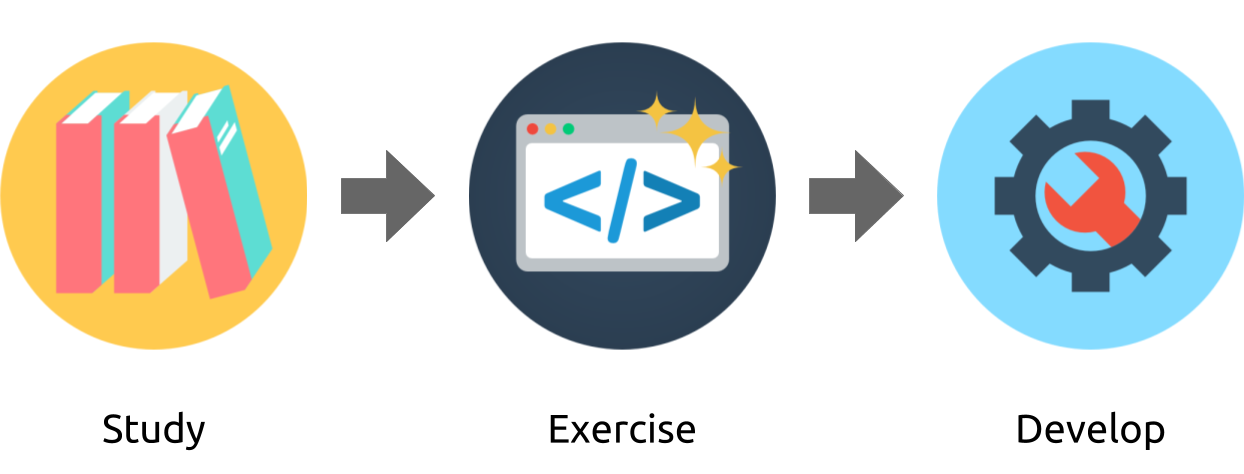
\includegraphics[width=1\textwidth]{immagini/fasi_progetto}
%	   	\caption{Le fasi principali del progetto di stage}
%	\end{figure}

\subsection{ELISE: Extended Loans Integrated System}
%In questa sezione parlerò abbastanza superficialmente del prodotto su cui la divisione in cui sono stato inserito lavora, ovvero ELISE, che è un applicazione web con scopo la gestione di finaziamenti.

	ELISE (Extended Loans Integrated System) è un software per cui la \textit{Business Unit} "793 - Servizi Finanziari e Assicurazioni" di Sopra Steria è commissionata, come molte altre aziende che forniscono consulenza nel dominio del \textit{banking}. La divisione infatti è tenuta allo sviluppo di nuove funzionalità e manutenzione su questo complesso sistema per un primario istituto di credito sul territorio nazionale, ovvero Banco BPM \footnote{Banco BPM. URL: \url{https://goo.gl/WkP9t6}}, gruppo bancario di origine cooperativa, presente in tutta Italia con l'eccezione dell'Alto Adige, operativo dal \ang{1} gennaio 2017. Questo istituto finanziario infatti è il risultato di una fusione di due grandi banche popolari, Banco Popolare di Verona e Banca Popolare di Milano, trasformatesi in S.p.A a partire dalla data di combinazione.\\

	\begin{figure}[H]
		\centering
	   	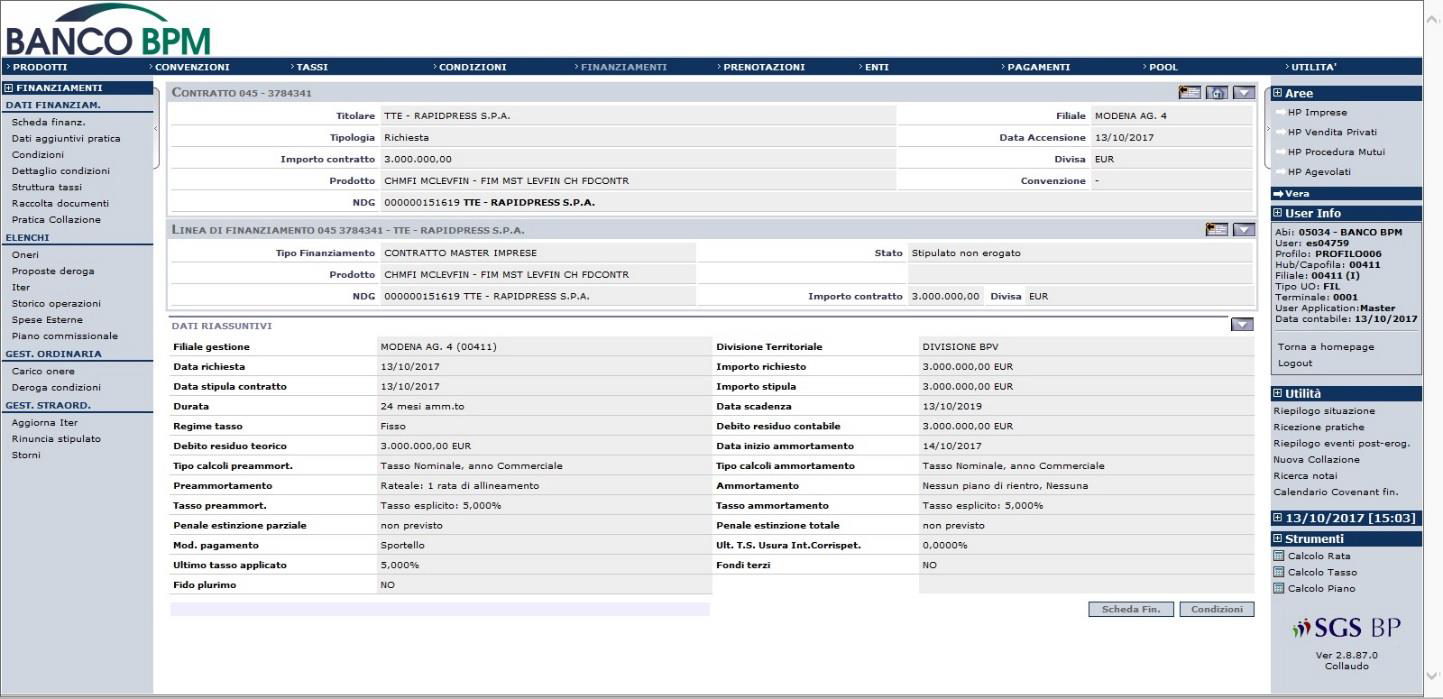
\includegraphics[width=0.85\textwidth]{immagini/Elise}
	   	\caption{Interfaccia dell'applicazione ELISE - Fonte: documento di collaudo interno aziendale}
	\end{figure}

	ELISE fornisce un ambiente completo che permette il tracciamento di un finanziamento da quando questo viene istanziato alla sua estinzione.\\
	
	ELISE si basa su un accesso ad utenza a cui sono predisposte delle abilitazioni. Ogni utente appartiene ad una filiale operativa e risulta responsabile di determinate attività da svolgere mediante l'applicazione, come ad esempio la richiesta finanziamenti, la verifica della documentazione, la gestione delle pratiche, le estinzioni, il pagamento rate, ecc. Normalmente gli utenti hanno solo determinate funzioni abilitate per sicurezza, la sede centrale invece possiede tutti i privilegi di operatività.\\
	
	I sistemi informativi di produzione in cui risiede l'applicazione web, sono in gestione presso una società ICT\glossario\ di terze parti. Tramite i loro server, il software è configurato alla comunicazione con un altro ambiente, quello di gestione dei dati, implementato su mainframe CICS\glossario\ basato appunto sulle transazioni dati.
		
%	\begin{figure}[H]
%		\centering
%	   	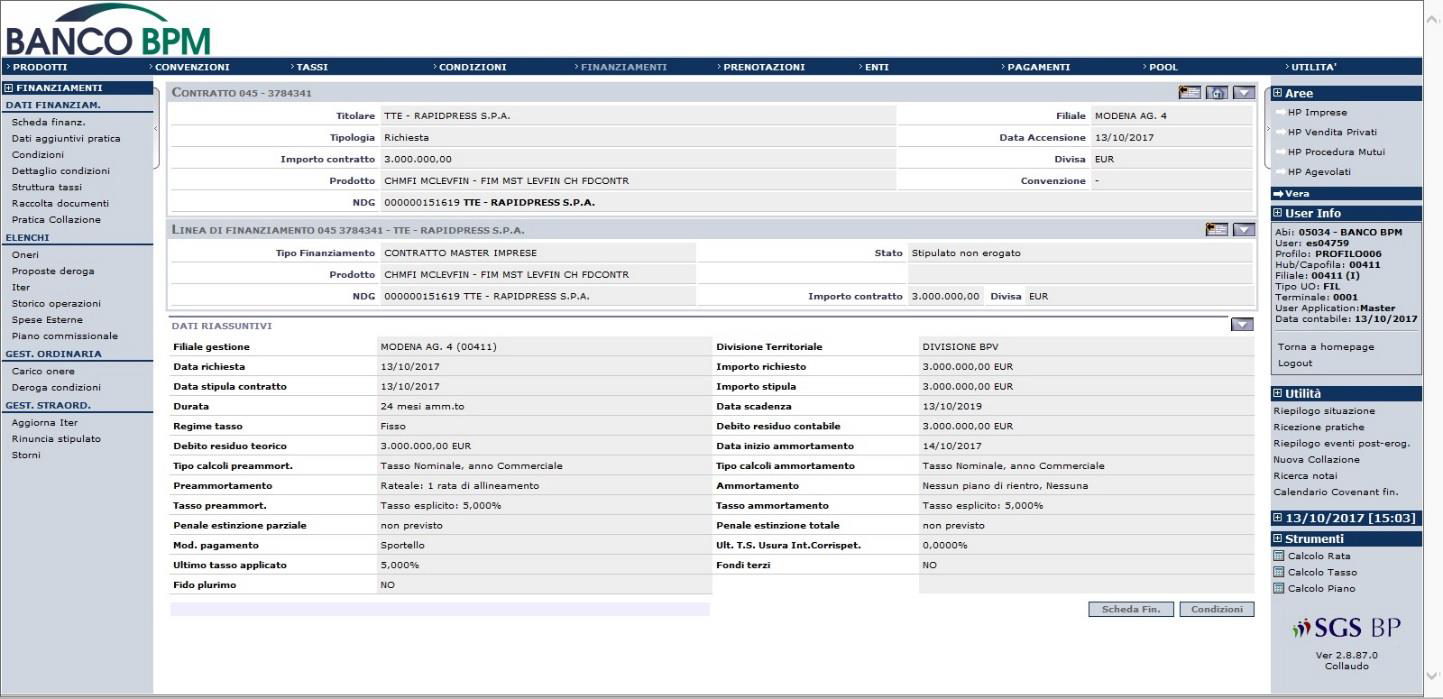
\includegraphics[width=0.85\textwidth]{immagini/Elise}
%	   	\caption{Interfaccia dell'applicazione ELISE - Fonte: documento di collaudo interno aziendale}
%	\end{figure}
	
	L'applicazione web offre, come principale strumento a supporto dei processi della banca, molteplici funzionalità, tra le più rilevanti:
	
	\begin{itemize}
		\item Prenotazione di finanziamenti sulla base dei tassi in vigore e dei dati forniti in input;
		\item Stipula dei contratti finanziari producendo in automatico come output l'accordo sottoscrivibile;
		%\item Richiesta di attivazione di un nuovo finanziamento a partire da uno prenotato; 
		\item Gestione di un finanziamento nei suoi passi, che fanno parte di quello che in ELISE viene chiamato \textit{iter pratica}, dalla prenotazione all'estinzione. Ciascuno di questi passi può essere abilitato solo per selezionate filiali della banca o tipologie di utenze;
		\item Gestione dei prodotti finanziari e dei loro parametri di periodicità, rateizzazione e spese di gestione da proporre ai clienti del gruppo bancario;
		\item Gestione dei tassi da applicare ai finanziamenti e della loro struttura fissa o variabile;
		%\item Gestione delle convenzioni stipulate per enti i cui parametri finanziari differiscono dal comune;
		\item Accesso a numerose utilità di amministrazione, calcolo di rate, tassi o piani di ammortamento\footnote{L'ammortamento è un procedimento contabile con il quale un costo pluriennale viene ripartito tra gli esercizi di vita utile del bene, facendolo partecipare per quote alla determinazione del reddito dei singoli esercizi. Nel nostro contesto rappresenta il piano di rateizzazione per il rientro del debito residuo sommato agli interessi calcolati} e vendita a privati, imprese e agevolati.	
	\end{itemize}
		
	\begin{figure}[H]
		\centering
	   	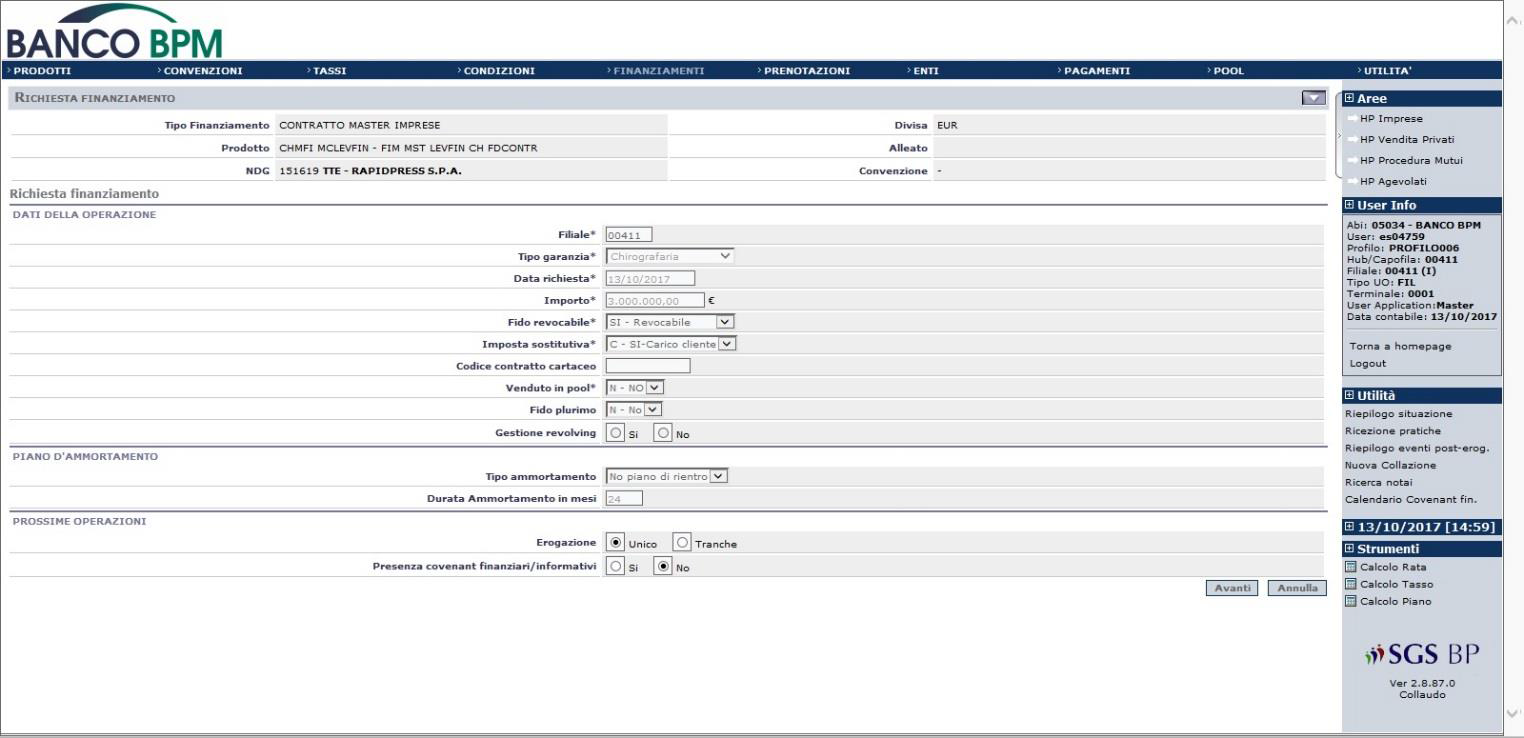
\includegraphics[width=0.85\textwidth]{immagini/RichiestaFinanziamento}
	   	\caption{Richiesta di finanziamento tramite ELISE - Fonte: documento di collaudo interno aziendale}
	\end{figure}
	
	Il portale viene utilizzato ogni giorno dai dipendenti di ogni filiale del gruppo bancario. Rappresenta quindi un mezzo di nota importanza per il cliente	e l'erogazione dei suoi servizi.

		
\section{Il mio stage}
%In questo inizio di sezione parlerò un po' di StageIT e dei progetti proposti dalle aziende in occasione di tale evento.

Le modalità con cui Sopra Steria Group S.p.A. attua alla ricerca di risorse sono molteplici, queste infatti possono andare dal reclutamento attraverso agenzie per il lavoro al reclutamento tramite \textit{social network} orientati al lavoro (come ad esempio LinkedIn\footnote{LinkedIn. URL: \url{https://goo.gl/nc4mVh}}), passando per il reclutamento per mezzo di eventi organizzati dalle università o dagli enti pubblici per agevolare l'incontro tra le aziende e gli studenti.\\

Quest'ultimo tipo di evento rappresenta la modalità con cui sono entrato in contatto con Sopra Steria, ovvero grazie al progetto Stage-IT\footnote{Stage-IT. URL: \url{https://goo.gl/UvdwLK}}, nella sua \ang{14} edizione che si è tenuta in data 5 Aprile 2017, dove le aziende hanno avuto modo di esporre i propri progetti e gli studenti le proprie ambizioni a far parte di essi. Stage–IT infatti è un'occasione di conoscenza reciproca per permettere agli studenti di avvicinarsi al mondo del lavoro e alle imprese di presentare la realtà in cui operano, illustrando le tematiche proposte per stage, con specifico riferimento al settore “\textit{Information and Communication Technology}" (ICT).\\

	\begin{figure}[H]
		\centering
	   	
\includegraphics[width=0.8\textwidth]{immagini/StageIT}
	   	\caption{Stage-IT 2017 - Fonte: \url{https://goo.gl/TqV3A6}}
	\end{figure}

\subsection{Proposte di stage}
%In questa sottosezione parlerò delle varie proposte di stage che ho ricevuto e dei progetti che proponevano.

Nei giorni successivi all'evento Stage-IT sono stato contattato da alcune delle aziende a cui avevo fornito il mio curriculum, in particolare quelle che più hanno mostrato interesse sono state Moku SRL\footnote{Moku SRL. URL: \url{https://goo.gl/exGzcj}} e Deloitte Italy S.p.A.\footnote{Deloitte Italy S.p.A. URL: \url{https://goo.gl/cUGDsp}}, oltre a Sopra Steria Group S.p.A. naturalmente.\\

Lo stage proposto da Moku SRL consisteva in un applicazione \textit{web} nell'ambito della sanità. Questo si poneva come obiettivo, inserendo lo stagista nel team di sviluppo lato front-end\glossario, formare una figura a scopo assunzione e far sì che questa veda un progetto crescere sin dalla nascita, partendo dalla progettazione sino al rilascio, e conseguente manutenzione nel tempo. Questo progetto di stage sarebbe stato molto interessante, soprattutto per le tecnologie che avrei potuto apprendere in un ambiente giovane ed innovativo come quello delle aziende facenti parte di H-FARM\footnote{H-FARM. URL: \url{https://goo.gl/Z2RVAE}}, che è un accelleratore di \textit{startup} che negli ultimi anni si è fatto sentire molto nel campo ICT. Purtroppo non ho potuto scegliere questo progetto perchè ho avuto la conferma da parte di Sopra Steria Group S.p.A. prima di quanto fatto da Moku SRL.\\
	\begin{figure}[H]
		\centering
	   	
\includegraphics[width=0.3\textwidth]{immagini/moku}
	   	\caption{Logo di Moku SRL - Fonte: \url{https://goo.gl/exGzcj}}
	\end{figure}

Lo stage proposto da Deloitte Italy S.p.A. consisteva invece in un implementazione all'interno del prodotto Microsoft Dynamics AX\footnote{Microsoft Dynamics AX. URL: \url{https://goo.gl/1N2jsA}}, che è un ERP\glossario\ che offre tutte le funzionalità centrali per la gestione di contabilità e finanza, risorse umane e operazioni necessarie per operare e trovare clienti su scala globale. Purtroppo non ho optato per questo progetto perchè la programmazione in ambito gestionali non mi ha mai appassionato, anche se l'azienda è una delle realtà più grandi su scala mondiale.\\
	\begin{figure}[H]
		\centering
	   	
\includegraphics[width=0.3\textwidth]{immagini/deloitte}
	   	\caption{Logo di Deloitte Italy S.p.A. - Fonte: \url{https://goo.gl/cUGDsp}}
	\end{figure}

\subsection{Motivo della scelta}
In questa sottosezione parlerò della scelta di stage che ho fatto e del motivo di tale scelta.

\subsection{Obiettivi del progetto}
In questa sottosezione parlerò degli obiettivi del progetto di stage che ho scelto.

\subsection{Vincoli del progetto}
In questa sottosezione parlerò dei vincoli imposti sia dall'azienda che dal cliente per il progetto di stage che ho scelto.

\subsection{Obiettivi personali}
In questa sottosezione parlerò degli obiettivi che mi sono imposto iniziando il progetto di stage.
